\subsection{Irregular Sensor Data Compression}
{{\footnotesize
\noindent This benchmark addresses lossy compression of irregularly sampled
sensor data from particle detectors using real-time autoencoder architectures,
targeting latency-critical applications in physics experiments.


\begin{description}[labelwidth=4cm, labelsep=1em, leftmargin=4cm, itemsep=0.1em, parsep=0em]
  \item[date:] 2024-05-01
  \item[version:] v0.2.0
  \item[last\_updated:] 2024-05
  \item[expired:] unknown
  \item[valid:] yes
  \item[valid\_date:] 2024-05-01
  \item[url:] \href{https://github.com/fastmachinelearning/fastml-science/tree/main/sensor-data-compression}{https://github.com/fastmachinelearning/fastml-science/tree/main/sensor-data-compression}
  \item[doi:] 10.48550/arXiv.2207.07958
  \item[domain:] Particle Physics
  \item[focus:] Real-time compression of sparse sensor data with autoencoders
  \item[keywords:]
    - compression
    - autoencoder
    - sparse data
    - irregular sampling
  \item[licensing:] Apache License 2.0
  \item[task\_types:]
    - Compression
  \item[ai\_capability\_measured:]
    - Reconstruction quality
    - compression efficiency
  \item[metrics:]
    - MSE
    - Compression ratio
  \item[models:]
    - Autoencoder
    - Quantized autoencoder
  \item[ml\_motif:]
    - Real-time, Image/CV
  \item[type:] Benchmark
  \item[ml\_task:]
    - Unsupervised Learning
  \item[solutions:] Solution details are described in the referenced paper or repository.
  \item[notes:] Based on synthetic but realistic physics sensor data

  \item[contact.name:] Ben Hawks, Nhan Tran
  \item[contact.email:] unknown
  \item[datasets.links.name:] Custom synthetic irregular sensor dataset
  \item[datasets.links.url:] \href{https://github.com/fastmachinelearning/fastml-science/tree/main/sensor-data-compression}{https://github.com/fastmachinelearning/fastml-science/tree/main/sensor-data-compression}
  \item[results.links.name:] ChatGPT LLM
  \item[fair.reproducible:] True
  \item[fair.benchmark\_ready:] True
  \item[id:] irregular\_sensor\_data\_compression
  \item[Citations:] \cite{duarte2022fastmlsciencebenchmarksaccelerating2}
\end{description}

{\bf Ratings:} ~ \\

\begin{tabular}{p{0.15\textwidth} p{0.07\textwidth} p{0.7\textwidth}}
\hline
Rating & Value & Reason \\
\hline
dataset & 5 & All criteria met
 \\
documentation & 4 & Setup for deployment (e.g., FPGA pipeline) requires familiarity with tooling
 \\
metrics & 5 & All criteria met
 \\
reference\_solution & 4 & Not fully documented or automated for reproducibility
 \\
software & 3 & Not containerized; Full automation and documentation could be improved
 \\
specification & 4 & Exact latency or resource constraints not numerically specified
 \\
\hline
\end{tabular}

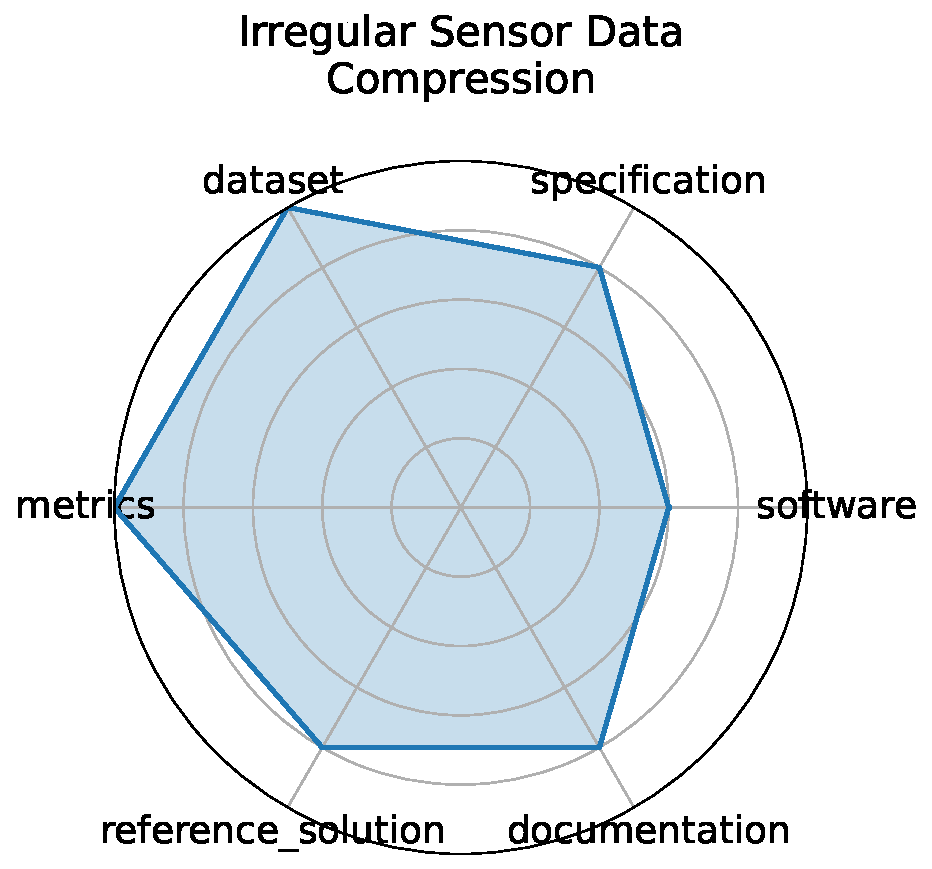
\includegraphics[width=0.2\textwidth]{irregular_sensor_data_compression_radar.pdf}
}}
\clearpage